\documentclass[a4paper]{article}
\usepackage{graphicx}
\usepackage{amsmath, amsfonts, geometry, float, listings, enumerate, multicol}
\usepackage{multicol, float, color, colortbl}
\usepackage{tikz, titlesec, parskip}

\titlespacing{\section}{0pt}{10pt}{0pt}
\titlespacing{\subsection}{0pt}{10pt}{0pt}
\titlespacing{\subsubsection}{0pt}{10pt}{0pt}

\usetikzlibrary{calc,patterns,through}
\newcommand{\arcangle}{%
	\mathord{<\mspace{-9mu}\mathrel{)}\mspace{2mu}}%
}

\renewcommand{\baselinestretch}{1.2}
 \geometry{
 a4paper,
 total={170mm,257mm},
 left=20mm,
 top=20mm,
 }
\usepackage{fancyhdr}
\pagestyle{fancy}
\fancyhf{}
\rhead{\textbf{مقدمه‌ای بر یادگیری ماشین}}
\lhead{\textbf{تمرین سری ششم}}
\cfoot{\space \space \space \space \textbf{\thepage}  \space \space \space}
\renewcommand{\headrulewidth}{1pt}
\renewcommand{\footrulewidth}{1pt}
 
\usepackage{xepersian}
%\setlatintextfont{Times New Roman}
\settextfont{XB Niloofar}
\setdigitfont{XB Niloofar}
\DefaultMathsDigits
\usepackage{amsmath}
\usepackage{pgfplots}
\tikzset{declare function={unitstep(\x)=notless(\x,0);}}
\tikzset{declare function={delta(\x)=equal(\x,0);}}

\begin{document}
\begin{minipage}{0.6\textwidth}

\begin{center}
	\begin{bf}
	باسمه تعالی\\
	\vspace{0.25cm}
	دانشگاه صنعتی شریف\\
	\vspace{0.25cm}
	دانشکده مهندسی برق\\
	\vspace{0.5cm}

\large
مقدمه‌ای بر یادگیری ماشین -دکتر سیّد جمال‌الدین گلستانی\\
\vspace{0.3cm}
\normalsize
بهراد منیری - ۹۵۱۰۹۵۶۴\\
\Large
\vspace{0.3cm}
گزارش  تمرین سری ششم\\
\vspace{0.4cm}

\end{bf}
\end{center}
\end{minipage} \hfill
\begin{minipage}{0.35\textwidth}

\begin{flushleft}
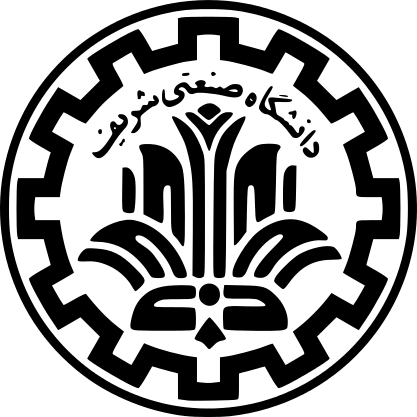
\includegraphics[width=0.6\textwidth]{Shariflogo.png}\\ \large
\end{flushleft}
\end{minipage}

\begin{large}
\section{مقدمه}
در این تمرین، از زبان پایتون برای پاسخ به سوالات استفاده شده و عمده‌ی توابع مورد استفاده از کتاب‌خانه‌ی
\lr{sklearn}
 هستند. 
 
در ابتدا، به کمک تابع
$\texttt{train\_test\_split()}$
داده‌های خود را به به دو بخش آموزش (۹۰ درصد) و تست (۱۰ درصد) تقسیم می‌کنیم. در تمام طول این تمرین، داده‌های تست توسط الگوریتم یادگیری ماشین دیده‌ نمی‌شوند و تنها برای  ارزیابی فرضیه‌ی منتخب توسط الگوریتم‌ یادگیری استفاده می‌شود.

ما از 
$\texttt{MLP Classifier}$
پیاده‌شده در کتابخانه‌ی مذکور استفاده خواهیم کرد. الگوریتم‌ یادگیری را 
\lr{Stochastic Gradient Descent}
قرار می‌دهیم با نرخ یادگیری‌ای برابر ثابت و برابر مقدار پیش‌فرض. همچنین تابع 
\lr{Activation}
را برابر 
\lr{ReLU}
قرار داده‌ایم.


\section{بررسی تاثیر تعداد قدم}
در این بخش، هشت لایه‌ی مخفی، هر کدام با هشت نورون، در نظر می‌گیریم. الگوریتم‌ یادگیری را ۵ بار با تعداد ‌قدم‌های 
$\{10,100,200,300,400\}$
اجرا می‌کنیم. 

\begin{figure}[h!]
	\centering
	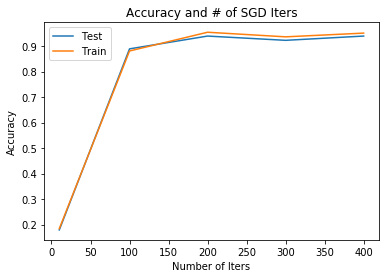
\includegraphics[scale=0.7]{1.png}
	\caption{اثر تغییرات تعداد استپ‌های گرادیان}
\end{figure}

مشاهده می‌شود که با افزایش تعداد گام‌ها، درصد صحت بر داده‌های تست و ترین افزایش می‌یابد. در شکل زیر، روند تغییر تابع
\lr{Loss}
را در هر یک از ران‌های فوق مشاهده می‌کنید.
\begin{figure}[h!]
	\centering
	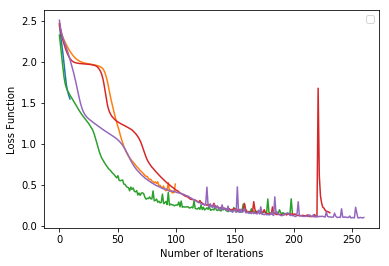
\includegraphics[scale=0.7]{2.png}
	\caption{مقدار تابع تلف بر حسب تعداد گام در پنج ران مختلف}
\end{figure}

\section{بررسی تاثیر عرض شبکه}
در این سوال به بررسی رابطه‌ی عمق شبکه و عملکرد آن بر روی داده‌های تست می‌پردازیم. 
شبکه‌ای با هشت لایه را با تعداد نورون‌های هر لایه‌ی 
$\{1,2,4,8,16,32\}$
آموزش می‌دهیم. تعداد گام‌های الگوریتم 
\lr{SGD}
را برابر ۱۰۰ می‌گذاریم. عملکرد این طبقه‌بند را بر داده‌های تست و ترین، بر حسب تعداد نورون‌های لایه‌ی مخفی، در شکل زیر مشاهده می‌کنید.
\begin{figure}[h!]
	\centering
	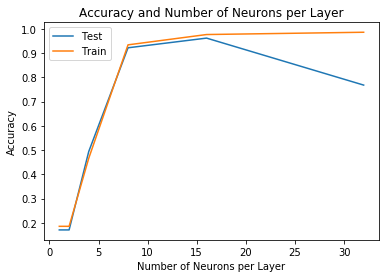
\includegraphics[scale=0.7]{3.png}
	\caption{عملکرد بر حسب تعداد نورون‌های هر لایه در پنج ران مختلف}
\end{figure}

نمودار مقدار 
\lr{Loss}
بر حسب تعداد گام نیز در شکل زیر آمده است.
\begin{figure}[h!]
	\centering
	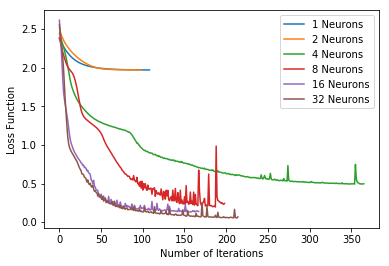
\includegraphics[scale=0.7]{4.png}
	\caption{مقدار تابع تلف بر حسب تعداد نورون‌های هر لایه در پنج ران مختلف}
\end{figure}
انتظار داشتیم که با افزایش تعداد نورون‌های هر لایه‌، عملکرد روی داده‌های ترین بهتر و بهتر شود که این اتفاق رخ داد اما انتظار داشتیم عملکرد روی داده‌های تست از جایی به بعد بدتر شود که به دلیل اینکه تعداد داده‌های آموزشی بسیار زیاد است این اتفاق رخ نداد.

در این بخش، ماتریس 
\lr{Confusion}
نیز رسم شده است تا درک بهتری از عملکرد طبقه‌بند داشته باشیم.
\begin{figure}[h!]
	\centering
	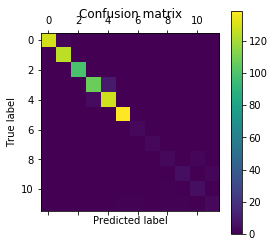
\includegraphics[scale=0.7]{conf.png}
	\caption{ماتریس کانفیوژن}
\end{figure}
\newpage
\section{بررسی تاثیر عمق شبکه}
در این بخش، تعداد لایه‌ها را افزایش می‌دهیم و نتایج بخش‌ قبل را مجدداً در این حالت نیز محاسبه می‌کنیم.
\begin{figure}[h!]
	\centering
	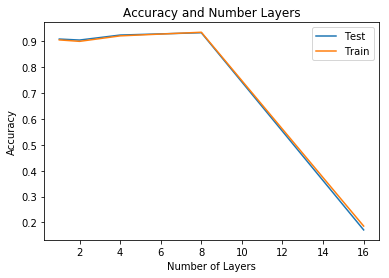
\includegraphics[scale=0.7]{7.png}
	\caption{عملکرد بر حسب تعداد لایه}
\end{figure}
\begin{figure}[h!]
	\centering
	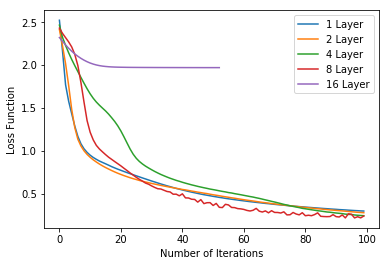
\includegraphics[scale=0.7]{8.png}
	\caption{تلف بر حسب تعداد لایه}
\end{figure}
\end{large}
در شکل ۷ دیده می‌شود که به دلایلی، در حالت ۱۶ لایه، الگوریتم 
\lr{SGD}
زود قطع می‌شود. 
\end{document}